%!TEX root = ../report.tex
\section{System context}
\label{sec:system-context}
The system context is a fundamental artifact in the software architecture of a system. Developing the system context view is important, because this view is used as a mechanism to trace back to the business context, and downstream to the functional and operational architecture.

\subsection{Diagram}
\label{subsec:system-diagram}
The system context diagram is outlined in \autoref{fig:system-context-diagram}. This diagram represents the different users and external parties that are involved in the SFM. In this diagram, the system is represented as a black box. In section 5.3 a more detailed view of the system is given. 

\begin{figure}[H]
	\centering
	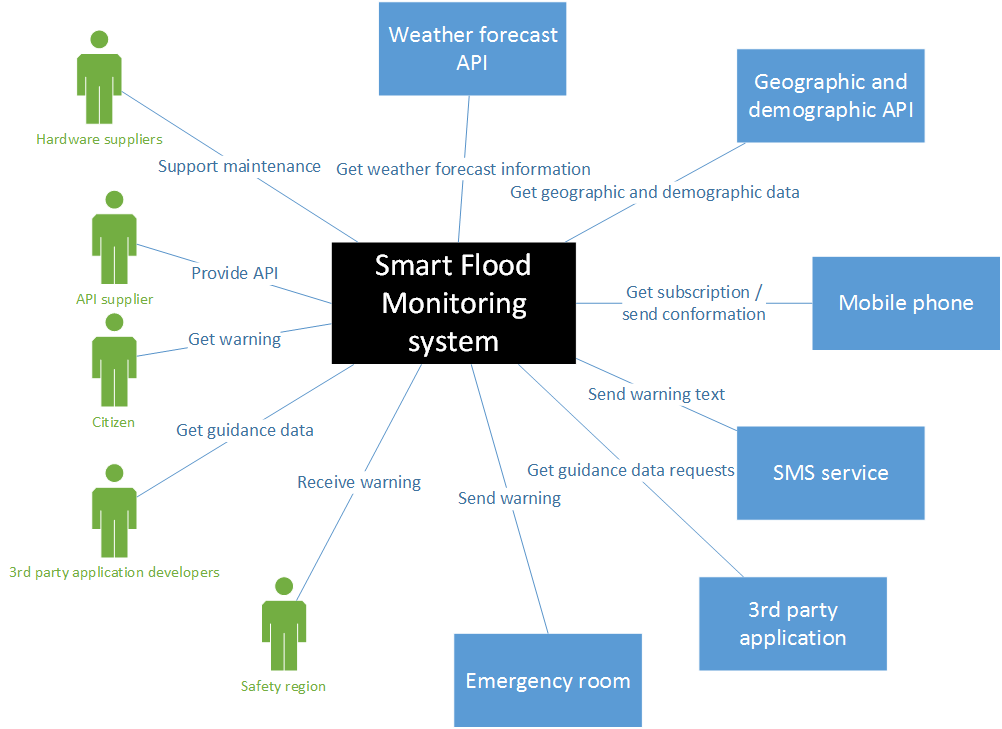
\includegraphics[keepaspectratio=true,width=0.7\textwidth]{images/system_context.png}
	\caption{System context diagram}
	\label{fig:system-context-diagram}
\end{figure}

Figure \ref{fig:system-context-diagram} only depicts external and internal connections. Internal user is not depicted in the diagram. However, internal users, such as system administrator and maintenance user, are able to connect to the system, which is authorized and authenticated using a password.

\subsection{Users and Roles}
\label{subsec:users-roles}
\begin{description}
	\item[Safety region] The safety region has the responsibility to protect citizens when a dangerous situation occurs. They receive a warning when there is an imminent flood. When the warning is received, the safety region can warn citizens and emergency services. The safety region needs information about time to evacuate, location and severity of the imminent flood.
	% \item[Citizens] Citizens can subscribe for receiving warnings in case of an imminent flood. Citizen will receive a warning when they are in an area which might get flooded. The warning consists of a message that they are in a dangerous area and should turn on TV or radio or surf to a safety region website in order to receive information how to protect yourself.
	\item[Third party application developers] This user will build an application to provide guidance when a flood is imminent. They use the data provided by the \gls{API} of the \gls{SFM}. They are allowed to get all relevant data from the system.
	\item[Hardware suppliers] This user will provide different kinds of hardware to the system and could act as a repairman when hardware is failing and can't be repaired right away.
\end{description} 

\subsection{External Systems}
\label{subsec:external-system}
\begin{description}
	\item[Weather Forecast API] The system will utilize weather forecast services from third party sources. To make this input reliable, the system uses multiple weather forecast providers. To predict floods correctly the system will need: rain data, temperature data, tides data, air pressure data and wind data.
	\item[Geographic and demographic API] To predict how floods will evolve over time, the system needs geographical data. There are multiple parameters that are needed by the system: ground height and waterways. To calculate the impact of an imminent flood on society, the system also needs to know how many people live in the affected area. This data is retrieved through the demographic API.
	% \item[Mobile phone] The mobile phone is a communication device of the citizen. This means a citizen uses the mobile phone to subscribe to the SMS service and to receive warnings in case of an imminent flood. This means the mobile phone should be able to send and receive text messages.
	\item[SMS service] The SMS system will communicate with the system and the mobile phones of the citizens. When a citizen wants to subscribe to the SMS service, the citizen can send a text message to the SMS provider containing the postal code and the house number. This data is then send to our system, which stores the information. When a flood is imminent and a warning needs to be issued, the system determines which citizens should receive a warning based on their address. The list of phonenumbers that is composed is then used to send a message to all citizens who are in the affected area. To do this, the SFM uses the API of the same SMS provider. If an imminent flood is detected, the warning text message to citizens arrives in five minutes.
	\item[Third party application] To guide citizens to a safe area in case of an imminent flood, we rely on third party applications. These applications get data from our API and deliver an app for citizens that provides guidance to a safe area.
	\item[Emergency room API] In case of an imminent flood we need to warn the safety region. This is done by invoking the emergency room API. In this way we send a message to the emergency room, which in their turn distributes this warning to the safety region. The safety region will be notified using TCP/IP channel (Internet). Thus, if an imminent flood is detected, the warning to the emergency room arrives within less than one minute.
\end{description}

\subsection{Channels and Information Flows}
\label{subsec:channels-information-flows}
This subsection elaborates channels and information flows from and to the \gls{SFM}. All connections are encrypted to ensure the security of the system.

\begin{table}[!htbp]
	\centering
	\begin{tabular}{L{\tw{0.3}} L{\tw{0.4}}}
		\toprule
		\multicolumn{2}{c}{$SFM\: \Leftrightarrow \: Weather \: forecast \: API$} \\ \midrule
		\textbf{Description}           & The system gets rain, temperature, tides, airpressure and wind data. \\
		\textbf{Connection}            & Wired, internet                                                      \\
		\textbf{Protocol}              & TCP/IP                                                               \\
		\textbf{Transaction occurence} & Real time                                                            \\
		\bottomrule
	\end{tabular}
\end{table}

\begin{table}[!htbp]
	\centering
	\begin{tabular}{L{\tw{0.3}} L{\tw{0.4}}}
		\toprule
		\multicolumn{2}{c}{$SFM \: \Leftrightarrow \: Geographic \: and \: demographic \: API$} \\ \midrule
		\textbf{Description}           & The system gets ground height data, waterway data and the amount of people who live in the affected area. \\
		\textbf{Connection}            & Wired, internet                                                                                           \\
		\textbf{Protocol}              & TCP/IP                                                                                                    \\
		\textbf{Transaction occurence} & Real time                                                                                                 \\
		\bottomrule
	\end{tabular}
\end{table}

% \begin{table}[!htbp]
% 	\centering
%     \begin{tabular}{L{\tw{0.2}} L{\tw{0.4}}}
%     \toprule
%     \multicolumn{2}{c}{$SFM \: \Leftrightarrow \: Mobile \: Phone$} \\ \midrule
%     \textbf{Description} & The mobile phone can subscribe to \\
%     \textbf{Connection} & Wireless, Internet \\
%     \textbf{Protocol} & 4G \\
%     \textbf{Transaction occurance} & Real time \\
%     \bottomrule
%     \end{tabular}
% \end{table}

\begin{table}[!htbp]
	\centering
	\begin{tabular}{L{\tw{0.3}} L{\tw{0.4}}}
		\toprule
		\multicolumn{2}{c}{$SFM \: \Leftrightarrow \: SMS \: Service$} \\ \midrule
		\textbf{Description}           & The SMS service receives subscriptions and sends warning messages to the right phone numbers when it gets warned by the system. \\
		\textbf{Connection}            & Wired, internet                                                                                                                 \\
		\textbf{Protocol}              & TCP/IP                                                                                                                          \\
		\textbf{Transaction occurence} & In case of an imminent flood                                                                                                    \\
		\bottomrule
	\end{tabular}
\end{table}

\begin{table}[!htbp]
	\centering
	\begin{tabular}{L{\tw{0.3}} L{\tw{0.4}}}
		\toprule
		\multicolumn{2}{c}{$SFM \: \Leftrightarrow \: Third \: party \: applications$} \\ \midrule
		\textbf{Description}           & The system will provide data to the third party applications through the API. \\
		\textbf{Connection}            & Wired, internet                                                               \\
		\textbf{Protocol}              & TCP/IP                                                                        \\
		\textbf{Transaction occurence} & Real time                                                                     \\
		\bottomrule
	\end{tabular}
\end{table}

\begin{table}[!htbp]
	\centering
	\begin{tabular}{L{\tw{0.3}} L{\tw{0.4}}}
		\toprule
		\multicolumn{2}{c}{$SFM \: \Leftrightarrow \: Emergency \: room \: API$} \\ \midrule
		\textbf{Description}           & The system warns the the safety region through the emergency room API. \\
		\textbf{Connection}            & Wired, internet                                                        \\
		\textbf{Protocol}              & TCP/IP                                                                 \\
		\textbf{Transaction occurence} & In case of an imminent flood                                           \\
		\bottomrule
	\end{tabular}
\end{table}


\subsection{Alternatives}
\label{subsec:system-alter}
\subsubsection*{Weather forecast data}
The system will use the openweathermap API. This is an API which can deliver both historical and forecast data. There are other options to get the current and forecast weather data, one of these options is forecast.io. We use this weather API if the openweathermap is unavailable. 

\subsubsection*{Geographic and demographic data}
The system will use the Nationaal Georegister (NGR) API to get the latest geographic data. To get the latest demographic data the system will use the open data from the Centraal Bureau van de Statistiek (CBS). This provider delivers both actual and historical data. It would also have been possible to download the data and import it just one time. However, the data needs to be up to date. This means the data needs to be updated once in a while, the easiest way to do this is by invoking the API.

\subsubsection*{SMS Service}
To warn the citizens in case of an imminent flood, we use the external CM Telecom SMS service. Citizens can subscribe to this service and receive a warning. Another option is that the system uses its own SMS service. The advantage of this is that we keep control of the process of warning citizens. However, it would be expensive to implement such a service. Besides this, outsourcing is more scalable since we don't have to cope with problems of sending text messages to other countries.

Another way of informing citizens would be to send a whatsapp message. However, all mobile phones are able to receive text messages, while not all mobile phones have internet access to receive whatsapp messages.  

\subsubsection*{Emergency room}
The emergency room will be warned by invoking their API. This decission was made to make sure all data will be received correctly. By warning the emergency room through telephone it would be possible the employee could accidently forget or change some of the information. If this would be implemented the SFM would need an employee 24/7, which is expensive. 

Another option is to send an email in case of an imminent flood. However, in this case it wouldn't be possible to continously update the information in the dashboard of the emergency service. This could also be achieved by continously sending mails, but this would take more time to open and interpret the emails.

